\hypertarget{sublime-natureza-e-cidade}{%
\subsection{Sublime, Natureza e
Cidade}\label{sublime-natureza-e-cidade}}

Debret, pintor de história oficial da corte portuguesa no Brasil, tem
sua produção atualmente mais reconhecida à margem das encomendas
oficiais, por meio da publicação do \emph{Voyage pittoresque et
historique au Brésil} (1834). Sua vista de Taubaté, registrada em
aquarela em 1827, é significativa de uma divergência ainda maior com
respeito à pintura oficial. Apresenta a cidade paulista numa grade
acanhada, não representativa da verdadeira fisionomia da cidade
\autocite{almanaqueurupes:2013arquiteto}, apequenada diante da escala da
paisagem natural (Figura \ref{fig:taubate}). O tema da natureza
sobrepujando a urbanização é, sabidamente, favorecido pelos viajantes
estrangeiros do século XIX, em obras como a célebre representação de
Ouro Preto por Thomas Ender (1817), o panorama de Vila Boa (Goiás) por
William Burchell (1827) ou a vista da Baía de Guanabara por Maria
Graham. É certo que tais imagens, tributárias do conceito de Sublime
oriundo do Romantismo europeu, sinalizam um espírito de exotismo
modelado no discurso iluminista de superioridade da natureza cultivada e
beneficiada pelos europeus, propalado pelo naturalista francês, o Conde
de Buffon (1707--1788) \autocite{palazzo:2002mitos}. No entanto, o tipo
figurativo da cidade em meio à natureza extrapola, em meados do século
XIX, o olhar condescendente dos viajantes europeus pela alteridade, para
ser adotado também pelos artistas brasileiros.

\begin{figure}
\hypertarget{fig:taubate}{%
\centering
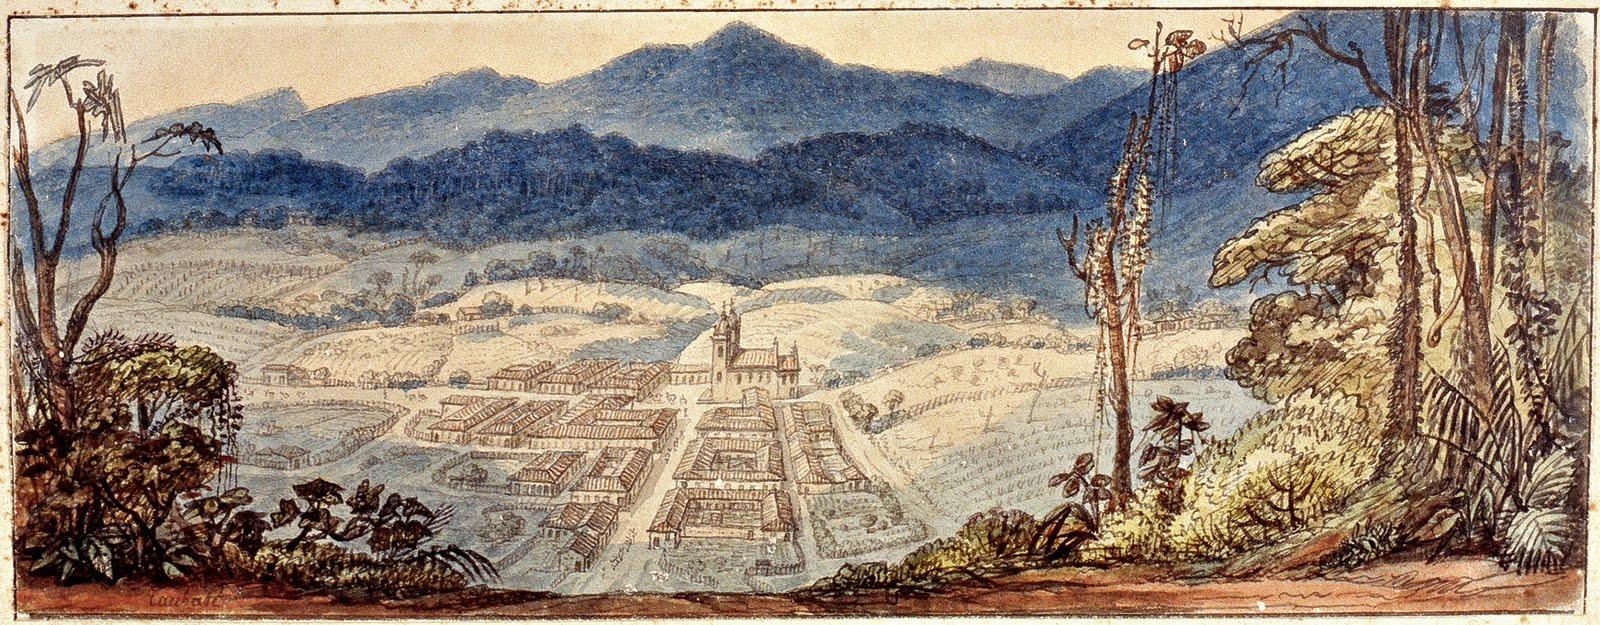
\includegraphics{figures/jb_debret_taubate.jpeg}
\caption{Jean-Baptiste Debret (1768--1848). Vista de Taubaté,
1827}\label{fig:taubate}
}
\end{figure}

Nas exposições gerais de belas artes, realizadas com periodicidade
irregular a partir de 1840, a pintura de paisagem só perde, em
quantidade de obras expostas, para os gêneros mais facilmente executados
do retrato e da natureza morta, mas deixa para trás a pintura histórica
e até mesmo a religiosa \autocite{squeff:2012galeria}. A paisagem do Rio
de Janeiro tomada do alto da Serra de Petrópolis, pintada em 1857 por
Agostinho José da Motta (1824--1878), explicita a fusão entre a pintura
de paisagem e o conceito de vista urbana como tema necessário à
afirmação nacional do Brasil (Figura \ref{fig:motta}). Nessa obra, a
cidade do Rio de Janeiro é apenas discernida pelo perfil de suas
montanhas no horizonte, eliminando-se qualquer indício de civilização em
prol da pujança geológica e florística.

\begin{figure}
\hypertarget{fig:motta}{%
\centering
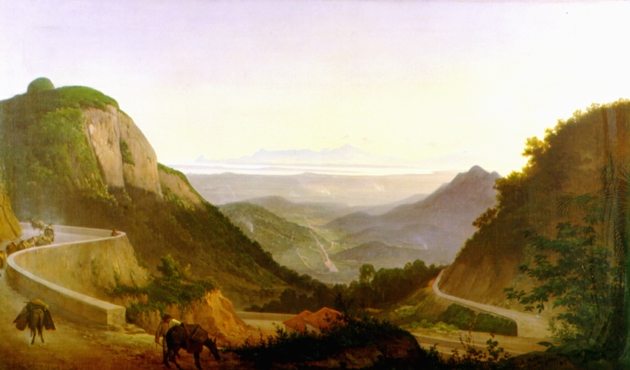
\includegraphics{figures/Agostinho_Jose_da_Mota_-_Paisagem_do_Rio_de_Janeiro.jpg}
\caption{Agostinho José da Motta (1824--1878). Paisagem do Rio de
Janeiro tomada do alto da Serra de Petrópolis, 1857}\label{fig:motta}
}
\end{figure}

Com o crescente mercado de estampas a partir do período regencial e,
mais tarde, de fotografias, a tipologia da vista urbana firma-se como
produto não apenas valorizado na Academia Imperial de Belas Artes
(AIBA), mas igualmente ao gosto do público, consumidor tanto de cenas da
vida cotidiana quanto de paisagens dos arredores da Capital ou das
províncias \autocite[p.~56]{turazzi:2009iconografia}. A produção
pictórica carioca, vinculada à herança deixada pelas obras dos Taunay
retratando a floresta da Tijuca, a lagoa Rodrigo de Freitas e outras
áreas suburbanas do Município da Corte, assume a idiossincrasia de
exaltar a cultura nacional por meio da afirmação de sua própria
insignificância perante a força da natureza.

A Exposição de História do Brasil, realizada no Rio de Janeiro em 1881,
não alinha em suas galerias de arte nada além de vistas da Capital, as
quais se distribuem entre o panorama urbano documental e as cenas da
pujante natureza e relevo entre os quais a própria cidade se perde. O
próprio \emph{Mappa architectural do Rio de Janeiro,} desenhado por João
da Rocha Fragoso e litografado em 1874, oferece, em vez da exuberante
natureza, cândida visão da Capital com seu tecido edificado de origem
colonial, patente confissão da pitoresca especificidade brasileira em
contraste com a grandiloquência das capitais europeias.

O prestígio artístico e crítico de Araújo Porto-Alegre alavancado em
prol do Romantismo, e as concomitantes campanhas etnográficas inspiradas
na missão do IBGE de se constituir as bases ideológicas da nação,
contribuem para fortalecer a busca por imagens representativas do
caráter nacional. Durante algum tempo, a iconografia da Guerra do
Paraguai catalisa esse ímpeto simultâneo pelo Sublime e pela glória do
Brasil. Nos últimos anos do Império, porém, recrudesce a insistência na
produção de uma arte pictórica de reconhecível caráter nacional, indo
além da glorificação romântica da natureza e do pitoresco.

A limitada produção pictórica das províncias não adere, num primeiro
momento, a esse movimento crítico de complementação da vista urbana
oficial pela paisagem sublime engolindo a escala da cidade. As vistas da
cidade de Porto Alegre durante a segunda metade do século XIX, assim
como a fotografia de Militão Augusto de Azevedo em São Paulo por volta
de 1860, conformam-se ao modelo da vista documental de caráter oficial
--- confronte-se com a diversidade de perspectivas tomadas pelo
fotógrafo Georges Leuzinger no Rio de Janeiro da mesma época. Mais
marcante ainda é o panorama do Desterro (Figura \ref{fig:desterro},
atual Florianópolis) executado em 1847 pelo jovem Victor Meirelles
(1832--1903), diretamente baseado na vista do Rio de Janeiro desde o
Morro de Santo Antônio, de Nicolas Taunay (1818). Trata-se, portanto, de
uma obra inserida na linhagem da vista urbana documental, recusando-se a
qualquer ruptura com a iconografia mais convencional, bem como,
reciprocamente, a qualquer aproximação com a incipiente tradição da
vista urbana romântica.

\begin{figure}
\hypertarget{fig:desterro}{%
\centering
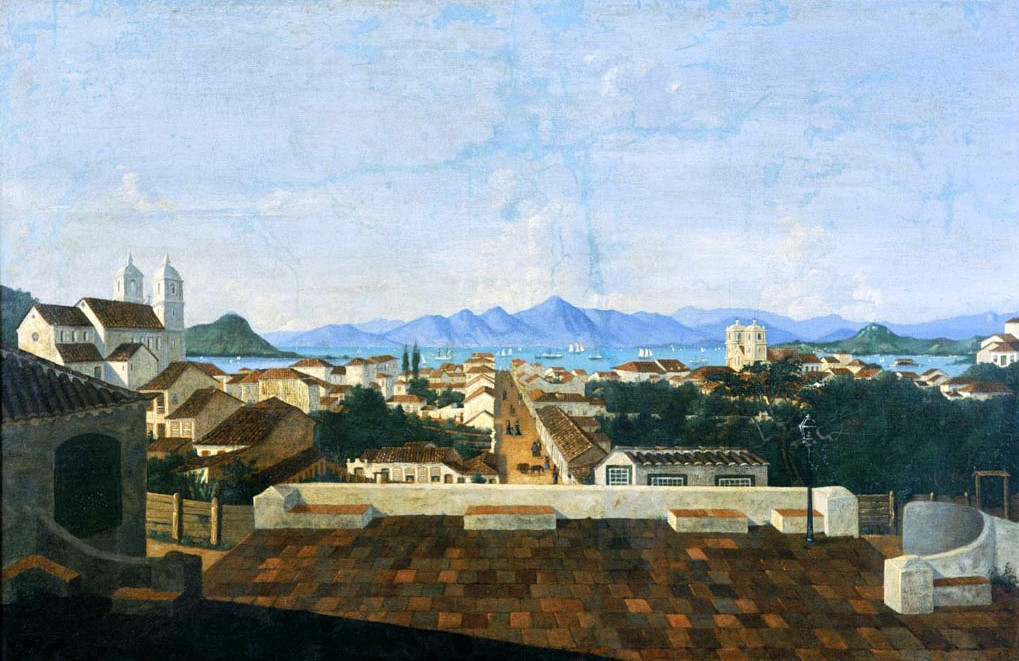
\includegraphics{figures/Victor_Meirelles_-_Vista_do_Desterro_-_c._1847.jpg}
\caption{Victor Meirelles (1832--1903). Panorama do Desterro,
1847}\label{fig:desterro}
}
\end{figure}
